% Anmerkungen:
%   Empfohlende Pakete:
%     cm-super für sauberere Schriftdarstellung

% Vorlagen
%   Pfeil als Randnotiz, der nach innen zeigt: \marginpar[\hfill$\Longrightarrow$]{$\Longleftarrow$}

\documentclass[
  fontsize=9pt
  ,paper=a5
  ,DIV=12
  ,BCOR=5mm
  ,abstract=true
  ,toc=bibliography
  ,toc=listof
  ,toc=index
  %,parskip=half
  ,twoside=true
  %,open=right
]{scrreprt}

% Fonts, Sprachunterstuetzung
\usepackage[utf8]{inputenc} %Deutsche Umlaute im Quellext
\usepackage[T1]{fontenc}
\usepackage{textcomp} %z.B. Währungssymbole (Euro €, Pfund Sterling £)
%\usepackage{lmodern}
\usepackage[ngerman]{babel} %Deutsche Silbentrennung, etc.
\usepackage{babelbib} %Mehrsprachige Literaturliste

% Graphiken und Farbe
\usepackage{graphicx} %Graphiken
\usepackage{color} %Farbe
\usepackage{pdfpages} %PDF-Seiten einbinden

% Mathematisches
\usepackage{amsmath}
\usepackage{amssymb} % mathfrak + amsfonts + spezielle Symbole
\usepackage{amsxtra} % Weitere Extrasymbole
\usepackage{mathrsfs} % \mathscr - normal ist \mathcal http://en.wikipedia.org/wiki/File:Mathscr-vs-mathcal.png
\usepackage{amsthm} % Definiert sind
%theorem, corollary, definition, definitions, fact, example,
%examples, Problem, Loesung, Definition, Satz, Beweis,
%Folgerung, Lemma, Fakt, Beispiel, and Beispiele.
%Beispiel: \proof{Ich habe etwas bewiesen.\qed}

% Mathematische Schrifterweiterungen
\usepackage{dsfont} %\mathds{A} alternativ zu mathbb
\usepackage{bm} %\bm{A} Boldface im Mathemodus

% Verbesserte Enumerate-Umgebung
%\usepackage{enumerate}
\usepackage[pointlessenum]{paralist} % siehe http://kaldor.vwl.uni-hannover.de/karl/ltxmp/latex.php

% Verbesserte Tabellen- und Equation-Umgebung
\usepackage{array}
\usepackage{eqnarray}
\usepackage{longtable}

% Diagramme
\usepackage[all]{xy}

\usepackage{url}
\usepackage{makeidx}
\usepackage{fancyhdr}

\definecolor{darkgreen}{rgb}{0,0.7,0} 
\definecolor{darkred}{rgb}{0.7,0,0} 
\definecolor{darkblue}{rgb}{0,0,0.7} 
\definecolor{lightgrey}{rgb}{0.97,0.97,0.97} 

% choco
%\definecolor{mycolor_background}{rgb}{0.1015625,0.05859375,0.04296875}
%\definecolor{mycolor_foreground}{rgb}{0.484375,0.64453125,0.38671875}
%\pagecolor{mycolor_background}
%\color{mycolor_foreground}

\usepackage[ngerman]{varioref}
%\usepackage[pdfborder=000, pdftex=true, plainpages=false, colorlinks=true, linkcolor=black, filecolor=black, urlcolor=black, citecolor=black, backref]{hyperref}
\usepackage[colorlinks=true,linkcolor=blue,citecolor=black,urlcolor=darkgreen]{hyperref}
\hypersetup{
	pdfpagelayout=TwoPageRight
	%,pdfstartview=Fit
}
\usepackage[ngerman]{cleveref}


%\usepackage[numbers,round]{natbib}
\usepackage[numbers,square]{natbib}
\bibliographystyle{alphadin}


\makeindex

\addtokomafont{caption}{\raggedright} % Bildunterschriften linksbündig

\newcommand{\todo}[1]{\textcolor{red}{TODO: #1}}
\newcommand{\degree}{\ensuremath{^\circ}}

%\renewcommand{\figurename}{Abbildung}
%\renewcommand{\tablename}{Tabelle}
%\renewcommand\contentsname{Inhaltsverzeichnis}


\newcommand*\myvref[1]{\nameref{#1}, \vref{#1}}
\newcommand{\mynote}[1]{\marginpar[\raggedleft\footnotesize #1]{\raggedright\footnotesize #1}}
\newcommand{\mynotetwo}[2]{\marginpar[\raggedleft\footnotesize #1]{\raggedright\footnotesize #2}}
\newcommand{\myindexednote}[1]{\mynote{#1}\index{#1}}



%\titlehead{fineshift M-Bus Reader v3.1.1 Dokumentation v2.0.0}
%\subject{Dokumentation\thanks{fineshift SLP-Rollout v1.4.1 Dokumentation v2.0.0}}
\subject{Manifest}
\title{Specios}
\author{Fabian Sandoval Saldias}
\date{17. Februar 2011}
%\publishers{fineshift \vtop{\vskip-25pt\hbox{\includegraphics[height=40pt]{gfx/fineshift.png}}}}
%\publishers{\textrm{}\vtop{\vskip-25pt\hbox{\includegraphics[height=40pt]{gfx/fineshift.png}}\vskip25pt} fineshift}
%\publishers{\textrm{}\vtop{\vskip-82.5pt\hbox{\includegraphics[height=160pt]{gfx/fineshift.png}}\vskip82.5pt}\textrm{}}
\publishers{\textrm{}\vtop{\vskip-43pt\hbox{\includegraphics[height=80pt]{gfx/fineshift.png}}\vskip44pt}\textrm{}}
%\dedication{Vielen Dank}



%\renewcommand{\subsectionmark}[1]{
%  \markright{\thesubsection{} #1}
%}

%\setcounter{secnumdepth}{4}
%\setcounter{tocdepth}{4}


\pagestyle{fancy} %eigener Seitenstil
%\renewcommand{\chaptermark}[1]{\markboth{\chaptername\ \thechapter\ #1}{}}
%\renewcommand{\sectionmark}[1]{\markright{\thesection\ #1}}
\renewcommand{\sectionmark}[1]{\markright{#1.\ \ \thesection}}
\fancyhf{} %alle Kopf- und Fußzeilenfelder bereinigen

\fancyhead[EL]{\textsc{\nouppercase{\leftmark}}} %Kopfzeile links
\fancyhead[OR]{\textsc{\nouppercase{\rightmark}}} %Kopfzeile rechts
%\fancyfoot[R]{\thepage} %Seitennummer
\fancyfoot[OR]{\thepage} %Seitennummer
\fancyfoot[EL]{\thepage} %Seitennummer
%\renewcommand{\footrulewidth}{0.4pt} %untere Trennlinie

\fancypagestyle{plain}{
  \fancyhf{} %alle Kopf- und Fußzeilenfelder bereinigen
  %\fancyfoot[R]{\thepage} %Seitennummer
  \fancyfoot[OR]{\thepage} %Seitennummer
  \fancyfoot[EL]{\thepage} %Seitennummer
  \renewcommand{\headrulewidth}{0pt} %obere Trennlinie
  %\renewcommand{\footrulewidth}{0.4pt} %untere Trennlinie
}


% Folgende Befehle machen den Veränderten Rand durch twoside=true wieder weg.
% Wird twoside=true nicht verwendet oder soll das ganze gebunden werden, sollten
% diese Befehle entfernt werden.
%\setlength{\oddsidemargin}{0cm}
%\setlength{\evensidemargin}{0cm}


\begin{document}


\dedication{%Für die armen Tieren auf dieser Welt.
Für Sissie.
}
\pdfbookmark{Startseite}{title}\maketitle


\pdfbookmark{\abstractname}{abstract}
\begin{abstract}
Unser Gesellschaftsmodell hat ausgedient. Wir werden von einer Minderheit beherrscht, welche natürlich alles tut, um ihre Machtposition zu behalten. Dies ist ein ganz natürliches Verhalten und wird durch unser profitorientiertes System sogar unterstützt. Vor der Industrialisierung war das sogar sinnvoll. Heute aber führt dies zu Massenversklavung, Wohlstandsverlust und riesiger Ressourcenvernichtung.

Dieses Manuskript wird diesen Wandel erklären, warum sich alternative Systeme wie der Kommunismus nicht etablieren konnten und warum eine Veränderung zwingend notwendig ist. Schließlich wird eine mögliche Lösung präsentiert: das Specios. Mit ihm wird ein grundlegend neues Gesellschaftskonzept vorgelegt und erläutert, wie es in wenigen Jahren alle derzeitigen politischen und Rechtssysteme erfolgreich unterwandern und ein nachhaltig wohlständiges Leben auf dem gesamten Planeten und darüber hinaus garantieren kann.

\end{abstract}


\pdfbookmark{\contentsname}{toc}\tableofcontents
%\clearpage


%\begin{enumerate}
% \item Erster Block. Hier wird die Marke gesetzt.\label{verweis}
% \item Mittels \pageref{verweis} kann auf die Seitennummer des fraglichen Labels verwiesen werden.
% \end{enumerate}


% \vspace*{10cm}
 % \begin{longtable}{|l|r|c|p{2cm}|}
 % \hline
 % Linksbündige Spalte.&Rechtsbündige Spalte&Zentrierte Spalte&Parbox\\
 % \hline
 % Kurzer Text.&Kurzer Text.&Kurzer Text.&Kurzer Text.\\
 % \hline
 % Text.&Text.&Text.&In diesem Felde nun ein elendslanger text, um Umbrüche innerhalb eines Feldes zu erzeugen.\\
 % \hline
 % Text.&Text.&Text.&der Befehl $\backslash$vspace*\{\} weiter oben im Quellcode hat einem Umbruch vor dieser Zeile bewirkt.\\
 % \hline
 % \end{longtable}


% \begin{enumerate}
% \item Zweiter Block. Hier wird nach \vref{verweis} verwiesen.
% \item Mittels \pageref{verweis} kann auf die Seitennummer des fraglichen Labels verwiesen werden.
% \end{enumerate}


% \section{Erster Abschnitt}\label{sec:firstsection}
% Wenn $a=2$ und $b=3$ dann gilt:
% \begin{equation}\label{eq:simpleeq}
% a+b =2+3=5
% \end{equation}
% Wie in \cref{eq:simpleeq} gezeigt \ldots
% \newpage
% \section{Zweiter Abschnitt}\label{zweiter Abschnitt}
% \Cref{eq:simpleeq}\vpageref{eq:simpleeq} verdeutlichte bereits \ldots


% So sind 96 \% der bundesdeutschen Schulen mit Computern ausgestattet. \cite[S. 7]{bmbf} ...


%\chapter{Übersicht}\label{chap:overview}

Dieses Kapitel bietet eine Übersicht über das System.

\section{Haupttabellen}

Die wichtigste Tabelle ist die "`Kunden"'"=Tabelle, in der alle Kunden mit allen nötigen Informationen, z.B. dem anzuwendenen Standardlastprofil, gelistet sind. Slp"=Rollout unterstützt Sie dabei, die Informationen über Kunden zu vervollständigen.

Die Tabelle "`Gesamtmengen"' enthält den gemessenen Gesamtverbrauch eines Kunden für jedes Jahr. Mit Slp"=Rollout können die Daten importiert werden.
Der Verbrauch der vergangenen 3 Jahre wird aus dieser Tabelle verwendet, um den Kundenwert zu berechnen. Der Kundenwert ist ein Maß für die Größe des Verbrauches im Verhältnis zu den mit Hilfe des Kundenmodells mathematisch berechneten Referenz"=Werten.

Die Tabelle "`Stundenwerte"' enthält die ausgerollten Verbrauchswerte eines Kunden für jede Stunde eines Jahres, mit einer Genauigkeit von 24h.

\section{Weitere Tabellen}

Der wichtigste Faktor bei der Schätzung des Verbrauchs ist die durschnittliche Tagestemperatur. Sie wird mit Hilfe von Wetterstationen erfasst, dessen Daten in der Tabelle "`Tagestemperaturen"' gepflegt werden müssen.

Jeder Eintrag in dieser Tabelle ist mit einer "`Temperaturquelle"' verknüpft, welche in der gleichnamigigen Tabelle hinterlegt wird.


Die Tabellen "`PLZBundelandZuordnungen"' und "`OrtBundelandZuordnungen"' dienen Slp"=Rollout zur automatisierten Zuordnung von Kunden zu den Bundesländern anhand der Postleitzahl oder des Ortes. Die Tabelle "`VertragsnameSLPZuordnungen"' enthält entsprechend Zuordnungen von Vertragsname"=Bestandteilen zu dem zu verwendenden SLP.

Die Tabelle "`Feiertage"' enthält alle festen (optional bundeslandspezifischen) Feiertage. Bewegliche christliche Feiertage berechnet das Programm selbstständig.

Alle anderen Tabellen beinhalten die von der TU München ermittelten Parameter für die SLP"=Ausrollung bzw. die Namen, die sich hinter Bundesland- und SLP"=Kennungen verbergen.

\section{Parameter, Auswirkungen}

Der ausgerollte Verbrauchswert eines Tages ist abhängig vom Bundesland, vom gewählten SLP und dessen Ausprägung (\verb|++|, \verb|+|, \verb|o|, \verb|-| oder \verb|--|), vom Wochentag/Feiertag, von der Durchschnittstemperatur und vom Kundenwert (siehe \vref{sec:rollout_mathematics}).

Das bedeutet, dass, wenn für einen ganzen Monat die selbe Temperatur angenommen werden würde, die einzige lokal greifende Variable der Wochentag wäre. Sofern keine Feiertage dazwischen liegen, würde sich das Verbrauchsschema also alle 7 Tage wiederholen, beim Ein- und Mehrfamilienhaushalt würde der Verbrauch sogar an jedem Tag des Monats identisch sein, da sie wochentagsunabhängig sind.

Kunden mit denselben Parametern (Bundesland, Temperaturquelle, SLP, SLP"=Ausprägung) haben relativ gesehen exakt dasselbe Profil, lediglich die Absolutwerte sind je nach Kundenwert unterschiedlich (aber gleichmäßig) skaliert.

%\begin{figure}
%\caption[Überblick/Datenbank]{Überblick über die vom Programm verwendeten Tabellen}
%\includegraphics[width=\textwidth]{gfx/overview_database.png}
%\label{fig:overview_database}
%\end{figure}
\chapter{Vorwort}\label{chap:prologue}

Wir wissen im Grunde alle, wie schlecht wir unseren Heimatplaneten behandeln. Wir nehmen bei unseren Aktionen kaum Rücksicht auf Langzeitfolgen, eher streben wir nach greifbarem Glück. In der Folge werden wertvolle Ressourcen ausgebeutet, die Flora und Fauna wird ausgerottet und unsere Lebensbedingungen pendeln sich in Extrema ein. Der Mensch kann mit dieser riesen Verantwortung, welche durch sein immenses Handlungspotenzial einhergeht, nicht wirklich umgehen.

Die restlichen Lebewesen bekommen das alles einigermaßen hin, da sie im Gegensatz zu uns in ihren Handlungsmöglichkeiten ziemlich beschränkt sind und die Umwelt genügend Zeit hat, auf Änderungen zu reagieren. Die Wesen passen sich durch evolutionäre Entwicklungen gegenseitig aneinander an. Die Macht der Intelligenz wird mit einem ausgeklügelten System aus Reflexen, Instinkten und schließlich Emotionen im Zaum gehalten. Ein Beispiel ist die Empathie unserer Mitmenschen gegenüber, was unterbewusst dafür sorgt, dass wir uns nicht gegenseitig auffressen oder Ähnliches. Je intelligenter und weitreichender Entscheidungen getroffen werden können, also je stärker diese "`eingebauten"' Regeln umgangen werden können, desto wichtiger werden externe Regeln, um das natürliche Gleichgewicht nicht zu stören.

Die Gesellschaft definiert solche Regeln in verschiedenen Ebenen. Von durch kulturellen Einflüsse in nächster Umgebung mitgegebenen moralischen Werten, welche meist auf den biologischen aufsetzen, bis hin zu weniger transparenten Gesetzen, welche komplexere Zusammenhänge berücksichtigen. Offensichtlich ist es aber ziemlich schwer, die tatsächlichen und relevanten Zusammenhänge zu erkennen und auch gehen die Meinungen diesbezüglich weit auseinander. Diesen Umstand möchte ich mit Hilfe moderner Informationsverarbeitung verbessern. Die Technik wird uns erlauben, gemeinsam optimale Regeln zu erstellen, welche den ursprünglichen Sinn derselben für uns extrapoliert: Die zerstörungsfreie Symbiose zwischen Mensch und Natur. Da Regeln alleine nicht viel nützen, ist die Konstruktion drumherum mindestens genauso wichtig.

Dies alles soll in der vorliegenden Arbeit besprochen werden. Für interessierte Leser sei angemerkt, dass sie keine Prosa enthalten wird. Gesellschaftssysteme sind komplex und viel diskutiert und bis heute ist es uns nicht gelungen, ein nachhaltig funktionierendes System zu entwickeln. Daher versuche ich so sachlich wie möglich zu bleiben, so dass Diskussionspunkte wohldefiniert sind und Kritik oder Verbesserungsvorschläge systematisch untersucht werden können.

Ich wünsche allen Lesern eine aufregende Zukunftsvorfreude.
\chapter{Einführung}\label{chap:introduction}

Dieses Kapitel wird den Hintergrund und die Notwendigkeit von einem grundlegend neuen Gesellschaftssystem verdeutlichen.

Verschiedenste Probleme sind allgemein bekannt:
\medskip
\begin{compactitem}
\item Hunger, Verschmutzung, niedrige Lebensqualität
\item Tierquälerei (Massentierhaltung mit allen Konsequenzen, Fischerei\footnote{Fische haben ein komplexes Schmerzbewusstsein analog zu Säugetieren, wie Studien der Gehirnaktivität und des Folgeverhaltens belegen. \citep{spiegel_10_2011}}, Pelz"=Beschaffung, überflüssige Tierversuche, Missbrauch für Unterhaltungszwecke)
\item Zerstörung der Natur (Abholzung, Ausrottung, Freisetzung fossiler CO\textsubscript{2}"=Einlagerungen, chemische und atomare Kontaminierung)
\item tödliche Auseinandersetzungen (Kriege, Terror"=Anschläge)
\item niedere Arbeiten
\item Überbevölkerung
\end{compactitem}
\medskip

Ein großer Fehler bei den meisten bisherigen Versuchen einer entsprechenden Problemlösungsstrategie oder zunächst einmal einer Ursachensanalyse innerhalb der Gesellschaftsordnung war der, nicht naturwissenschaftlich an das Problem heranzugehen; geblendet von Religionen und klassischen Ideologien. Es fängt bei der Argumentation an, was denn das Ziel für die Gesellschaft und den einzelnen Menschen darstellen soll, welche nur auf Grundlage willkürlicher Moralvorstellungen oder überhaupt nicht geführt wurde.

\section{Situation}\label{sec:situation}

Dieser Abschnitt wird die derzeitige Gesellschaftssituation verdeutlichen, warum wir hier gelandet sind, warum es scheinbar ganz gut funktioniert, warum bisherige Änderungsversuche scheiterten und warum das auf keinen Fall so bleiben darf.

\subsection{Kapitalismus}\label{sec:situation/capitalism}

Wir leben im Kapitalismus. Selbst sozialistische Staaten wie China, Nordkorea, Vietnam oder Kuba sind in die globale Marktwirtschaft eingebunden und eigentlich eher kapitalistisch. Zumindest kann nicht bestritten werden, dass jeder irgendwie nach Geld giert.

Wird man davon glücklich? In unserem System eine klare Antwort: "`ja"'. Gesundheit, Spaß, Zeit. Alles kostet Geld und die meiste Arbeit heute dient einzig der Vermehrung von selbigem. Wenn man das Tauschmittel Geld nur oberflächlich betrachtet, macht es natürlich Sinn: Als Jäger und Sammler konnten wir noch eigentumslos leben, alles wurde in der Gruppe aufgeteilt. Später entwickelte man aber den Ackerbau und die Viehzucht, wurde sesshaft. Bauern waren in der Lage mehr Nahrung zu produzieren als sie selbst benötigten, ihnen fehlten dafür aber andere Dinge; der Tauschhandel begann. Um die Suche nach einem Tauschpartner zu vereinfachen, die teilweise geringe Haltbarkeit der Tauschgüter zu umgehen und die Frage nach dem Gegenwert zu verallgemeinern, wurden später möglichst seltene und lang haltbare Zwischentauschmittel eingeführt, wie z.\,B. Kaurischneckenhäuser in China irgendwann zwischen dem 7. und 11. Jahrhundert vor Christus \citep{yungti_2003}. In der Folge wurden daraus Gold"~ und Silber"=Münzen mit entsprechendem Gegenwert\footnote{Häufig war der Wert einer Münze etwas höher als die enthaltenen Metalle, um den Herstellungsaufwand einzubeziehen und ein Wiedereinschmelzen unattraktiver zu machen.} bis man sich schließlich von der Notwendigkeit eines Warenwertes trennte, wie es bei unserem heutigen Bar"~ und Buchgeld der Fall ist. Das klingt zunächst wie eine perfekte Lösung.

Ein großes Problem ist die Verwaltung des Geldes. Heutzutage wird es vermehrt ohne einen echten Gegenwert zu haben. Durch das Zinssystem gibt es immer mehr Schulden als (virtuelles) Geld, d.\,h. die ganze Welt kann den privatisierten Banken gegenüber insgesamt niemals schuldenfrei sein. Großkonzerne und Banken haben Geld und demnach Macht über jeden, der Geld benötigt. Nicht nur normale Bürger, auch die Regierungen gehören dazu. Folglich bringt es rein garnichts in die Politik zu gehen, wenn man etwas daran ändern möchte -- die sogenannte "`Elite"', wie sie Verschwörungstheoretiker nennen, wird das verhindern. Das ist nur leider keine Verschwörungstheorie sondern eine Tatsache. Die genauen Verhältnisse kann man überall selbst nachlesen.

Ein weiteres entscheidendes Problem ist relativ jung. Wir sind an einem Punkt angelangt, an dem wir die gesamte Welt problemlos versorgen könnten.\footnote{Siehe dazu auch die Ergebnisse des \textit{Venus"=Projektes}.} Doch alles was man zum Leben benötigt kostet Geld und Geld bekommt man nur durch Arbeit. Wie schafft man sich Arbeit, wenn es eigentlich kaum welche geben muss? Man produziert billig und kurzlebig. Man sorgt künstlich für Knappheit, denn was selten ist, ist wertvoll. Beispielsweise werden in der Kimberly Diamantenmine Diamanten verbrannt, um den Preis hoch zu halten. Darüberhinaus lässt man monotone und anspruchslose Arbeit von Menschen statt von Maschinen erledigen um die Arbeitslosenzahlen niedrig zu halten, denn man braucht ja Arbeit, um zu leben -- selbst wenn sie vollkommen sinnlos ist. Effizienz, Reichhaltigkeit und Nachhaltigkeit widersprechen folglich der Struktur des profitorientierten Systemes.

Das Wohl eines Menschen darf demnach nicht davon abhängen, möglichst viel Profit zu erwirtschaften oder allgemein gesagt Probleme zu lösen, denn sonst erzeugt er sie künstlich (wie Krieg oder Nahrungsmittelvernichtung).

\subsection{Arbeit}\label{sec:situation/work}

Ich führe nun den letzten Gedanken des letzten Abschnittes fort. Man soll demnach nicht arbeiten müssen, um ein Mindestwohlstandslevel zu erhalten. Für Luxusgüter wäre dies dagegen denkbar. Die Frage, die sich dabei auftut ist folgende: Wie soll die Welt funktionieren, wenn niemand arbeitet? Ein Punkt wurde bereits erwähnt und ist erheblich: Fortschritt und damit auch Automatisierung wird durch Patente oder sinnlose (es gibt auch sinnvolle) Parallel"~ oder Neuentwicklungen derselben oder bereits existierender Technologien bzw. Produkte erschwert. Oft sind Maschinen in unserem Wirtschaftssystem auch einfach nur unwirtschaftlich; eine Eigenschaft, welche in einem nicht"=monetären System gänzlich anders definiert wäre (die Grenzen wären nicht das Kapital und die eigenen Kompetenzen sondern lediglich die tatsächlich vorhanden Ressourcen und das Ziel wäre nicht die lokale Maximierung von Profit unter Anwendung diverser Tricks und Manipulationen auf Kosten des Gesamtwohles, sondern die direkte und tatsächliche Maximierung des Gesamtwohles.

Ein weiterer Punkt ist die falsche Annahme, dass wir nur für Geld arbeiten. Es gibt genügend andere Motive. Dies beweist beispielsweise die Tatsache, dass sich sogar jetzt schon etwa 10--40\% der Konsumenten meist ohne direkte materielle Gegenleistungen an (Weiter"~)""Entwicklungen, Modifikationen und Verbesserungen von Produkten beteiligen \citep[S.~11]{piller_oi_2006}. Folgende Beweggründe sind dafür verantwortlich \citep[SS.~11--13]{piller_oi_2006}.
\begin{compactitem}
\item Extrinsische Motive (Selbstnutzungserwartung).
\item Intrinsische Motive (Befriedigung des Spieltriebes (Spaß, Kreativität) und des Forschungsdranges verbunden mit dem Erreichen eines Flow"=Zustandes (Fesselung von der Arbeit), sofern eine erfüllbare Herausforderung erkannt wird; eine direkte Leistungsrückkopplung steigert den Effekt).
\item Soziale Motive (Anerkennung der eigenen Arbeit (von anderen Menschen, insbesondere von Mitarbeitern oder einer entsprechenden Community) und gegenseitige Unterstützung).
\end{compactitem}
Das Potenzial wird auch anhand einer Studie deutlich \citep{hippel_2010}, nach der sich 6,2\% der britischen Verbraucher an Innovationsprozessen beteiligten\footnote{Beobachtet wurde ein Zeitraum von drei Jahren.}, d.\,h. entweder eigene Produkte geschaffen oder bestehende angepasst haben. Die jährlichen Aufwendungen der Verbraucher entsprachen dabei dem 2,3"=fachen der Forschungs"~ und Entwicklungskosten aller britischen Unternehmen für Verbrauchsgüter.
%(vgl. auch die Entwicklung von \textit{Closed Innovation} zu \textit{Open Innovation})

\subsection{Gesetze}\label{sec:situation/laws}

Jedes Lebewesen ist im Kern egoistisch, das ist biologisch überlebensnotwendig. Allerdings muss es mit der Umwelt auf gewisse Weise kooperieren, wenn es überleben will\footnote{\textit{Überleben} als obersten Willen darzulegen ist nicht ganz korrekt, genügt aber hier. Das tatsächliche Lebensziel wird in \myvref{sec:basis/aim} behandelt.}. Folglich muss sich ein Organismus einschränken und kontrollieren, um mit anderen erfolgreich zu interagieren. Diese symbiotischen Beziehungen werden komplexer, je wirkungsvoller und weitreichender (auch zeitlich) sie ausgelegt sind und können von einem Organismus ohne weiteres nicht vollständig überschaut werden. Daher sind (global) einzuhaltende Regeln erforderlich, um letzlich das eigene Wohl sicherzustellen. Aus diesem Grund haben sich auch Grundbedürfnisse und Instinkte ausgebildet und sind wir Rudeltiere geworden: Unsere Vorfahren haben sich in Gruppen überschauberer Größe organisiert. Evolutionstechnisch ist es daher auch nicht abwegig, Fremde zunächst als Feinde zu betrachten. Folglich wirkt Altruismus höchstens in einem Familien"=Clan.

Die durch unsere Gesetze und Verhaltensweisen derzeit eher destruktive Beeinflussung der Welt liegt darin begründet, dass wir unsere vererbten Verhaltensweisen dank komplexer Lernfunktionalitäten in immer kürzerer Zeit umgehen können. Das unausweichlich eingeschränkte Gesamtbild, Ignoranz bzw. Egoismus und damit Machtgier sind hierbei grundlegende Faktoren für die Fehlentwicklung. Bisher konnte sich die Natur bei solchen extremen Abweichungen durch genetische Anpassungen immer selbstständig die Waage halten. Seit der Mensch aber so "`vehement viel denkt"', laufen die Veränderungen viel zu schnell und in einem zu großem Maßstab ab, wobei er die Auswirkungen selbst erst jetzt zu überblicken vermag.

\subsection{Demokratie}\label{sec:situation/democracy}

Es wird allgemein behauptet, dass wir in einer Demokratie leben. Tatsächlich haben wir aber kaum Einfluss auf Entscheidungen. Wir wählen Parteien, welche anschließend machen was sie wollen. Wäre dies nicht der Fall und würden sie für das Allgemeinwohl des Volkes arbeiten, würde nicht so viel Elend in der Welt herrschen, das genügt hier als Beweis.

Der Sinn dahinter war, dass Entscheidungen heruntergebrochen werden um die Komplexität zu verringern. Allerdings gehen übergeordnete Instanzen genauso wenig auf untergeordnete ein, wie Parteien auf die Bürger eingehen. Hier und da gibt es zwar Regeln, allerdings werden sie immer weiter aufgeweicht, hauptsächlich mit Hilfe psychologischer Manipulation, wodurch untergeordnete Instanzen, vor allem normale Bürger, diversen Initiativen quasi aus dem falschen Bauchgefühl heraus zustimmen. Dazu zählt insbesondere der Terror"=Hype. Seine Folgen sind beispielsweise die Lockerung des Datenschutzes inkl. steigender Überwachung oder die Aushebelung des deutschen Gesetzgebungsverfahrens durch den Vertrag von Lissabon.

Allzu direkt darf die Demokratie jedoch auch nicht sein. Als einfacher Bürger kann man die Komplexität hinter den Entscheidungen garnicht überblicken und handelt oft voreingenommen. Die Aufgabe der Parteien und Lobbyisten ist es, komplizierte Sachverhalte zu analysieren und Lösungen mit entsprechenden Begründungen vorzuschlagen, welche dann akzeptiert werden können oder nicht. Entscheidungen beruhen also auf dem Vertrauen weniger Instanzen, welche dieses natürlich zu ihren Gunsten ausnutzen können.

\subsection{Revolutionen}\label{sec:situation/revolutions}

Versuche, den von Karl Marx und Friedrich Engels prophezeiten Kommunismus durchzusetzen scheiterten schon an der sozialisitischen Vorstufe und am Wirtschafts"=Management.

Allgemein scheitern Revolutionsversuche, welche keine Diktatur hervorbringen wollen, an der Trägheit der Menschen. Die an den wichtigen Positionen zu wohlhabende und allgemein müde Masse beginnt nicht auf Basis von systemfeindlichen Diskussionen, sich rückhaltlos dem gewöhnlichem Alltag zu widersetzen, geschweige denn kollektiv und ausreichend konsequent. Dies wäre existenzgefährdend. Es müsste schon gewaltiges schief laufen, allerdings ist dies sehr unwahrscheinlich: Man will seine Sklaven schließlich behalten. Die "`Elite"' wird uns füttern, gerade so viel, dass wir arbeiten können und mangels Alternativen auch arbeiten werden.

Den letzten Punkt kann man gut anhand eines Spielkasinos verdeutlichen: Wir sind quasi die Spieler und die Politiker sind maximal die Croupiers. Warum sollten die Besitzer des Kasinos -- Großkonzerne und Banken -- etwas an den Regeln ändern? Oder gar das Kasino für alle freigeben? Es läuft für sie nunmal so wie es läuft.

\subsection{Analyse}\label{sec:situation/analysis}

Wir stellen also fest:
\begin{itemize}
\item Eine profitorientierte oder ressourcen"=arme Gesellschaft erzeugt Gier und damit Machtstreben. Ersteres bedingt der Kapitalismus und letzteres wird für ihn konstruiert.
\item Allgemeingültige Selbstlosigkeit bzw. Solidarität ist nicht angeboren.
\item Absolute Demokratie führt zu Chaos und benachteiligt Randgruppen; abgeschwächte Demokratie führt zum Kontrollverlust.
\item Wir werden in unseren Handlungsmöglichkeiten immer weiter eingeschränkt. Schon jetzt sind wir Sklaven, aber noch arbeiten wir unter freiem Himmel.
\item Wir sind technologisch so gut wie festgefahren. Noch länger auf einen Durchbruch zu warten, welcher uns zu einem besseren System befähigt, ist zu riskant.
\item Die Organisation bzw. der Aufruf zu revolutionären Tätigkeiten darf nicht von einer Minderheit ausgehen
\end{itemize}

Zusammenfassend kann man sagen, dass unser System grundlegende Widersprüche aufweist und Änderungen im benötigen Maßstab in ihm nicht möglich sind; wählen gehen genügt nicht. Man muss ganz von vorne beginnen. Mit den politischen Mitteln, die uns zur Verfügung gestellt werden, kommen wir nicht weiter. Die bloße Verteilung von aufklärenden Informationen genügt aber auch nicht.
\section{Konsequenzen}\label{sec:consequences}

In diesem Abschnitt werden die Konsequenzen aus der in \vref{sec:situation} dargelegten Situations-Analyse gezogen, welche die notwendigen Anforderungen an die Gesellschaftsrevolution definieren.

\subsection{Anforderungen}\label{sec:consequences/requirements}

Folgende Anforderungen müssen erfüllt werden, um einen erfolgreichen Wandel herbeizuführen:
\begin{itemize}
\item Massive Verhaltensänderungen oder massive Proteste gegen gegenwärtige Ideologien müssen organisiert und konsistent ablaufen.
\item Es muss viel bessere Aufklärungsarbeit geleistet werden -- flächendeckend, logisch und einfach nachvollziehbar.
\item Die Regeln müssen jederzeit von jedem nachvollziehbar sein und in Frage gestellt werden können.
\end{itemize}

\subsection{Synthese}\label{sec:consequences/synthesis}

Aus den Anforderungen folgt folgende notwendige Ideologie:
\begin{itemize}
\item Jegliche Meinungen der Menschen müssen in Relation zu ihrer Kompetenz auf dem themasierten Gebiet betrachtet werden und das System direkt beeinflussen.
\item Man benötigt ein Werkzeug, welches (komplexe) Zusammenhänge sowohl verdeutlicht als auch verifiziert.
\item Das gesamte System muss transparent über das Internet erfassbar sein.
\item Konsistenz, Korrektheit und Nachvollziehbarkeit wird durch Selbstdefinition der Regeln anhand so elementarer Entscheidungen wie möglich gewährleistet. 
\end{itemize}

Es ist also ein (wenn man so will im wahrsten Sinne des Wortes diktatorisches) Computersystem erforderlich, dessen "`Gehirn"' von der Menschheit demokratisch aufgebaut wird und dadurch nicht korrupt werden kann. Sämtliche abstrahierten/""finalen Entscheidungen sind demnach architektonisch bedingt von der Bevölkerung gedeckt und können jederzeit durch Argumentationsarbeit (Erweiterung/""Korrektur des Wissens des Systemes) angepasst werden. Zu den Anpassungen zählen nicht nur einfache Daten sondern auch Formeln, welche Zusammenhänge definieren.

Um nicht am Konservatismus zu scheitern muss eine möglichst vollständige Zielvorstellung vorgelegt werden. Dies kann am effektivsten mit dem Aufbau eines virtuellen Parallelsystemes erfüllt werden, welches die Vorteile und Wege klar präsentiert und somit auf Basis der Einsicht und Akzeptanz fließend angewendet werden kann. Die herrschende Minderheit wird auf diese Weise moralisch gezwungen sein, die Weichen entsprechen zu stellen und schließlich gewaltlos entmächtigt.

\chapter{Konzept}\label{chap:concept}

Dieses Kapital wird eine Lösung skizzieren, welche die in \vref{sec:consequences} dargelegten Anforderungen erfüllt.

Ich nenne das System \textit{Specios, la specio sistemo}\footnote{"`Specios, la specio sistemo"' (epo.\index{Esperanto}) bedeutet "`Specios, das Arten"=System"', wobei \textit{Art} im Sinne von \textit{Spezies} zu verstehen ist, und \textit{System} u.\,A. im politischen Sinne. Also ein Verwaltungssystem für jede Art von Lebewesen. Wenn man möchte, kann man \textit{Specios} selbst auch ähnlich eines rekursiven Akronyms betrachten, es steht für "`\textbf{Specio} \textbf{s}ystemo por \textbf{s}inkonservo, \textbf{p}rospero, \textbf{e}galrajteco kaj la \textbf{c}elado al \textbf{i}dentigado de \textbf{o}bskureco"' (epo.\index{Esperanto} Arten"=System zur Selbsterhaltung, Wohlstand, Gleichberechtigung und dem Bestreben nach der Identifizierung der Unbekanntheit). Zu beachten ist, dass "`specios"' nicht esperanto ist, bezeichnet also auch nicht die Mehrzahl von "`specio"', dies wäre "`specioj"'.}.

\section{Grundlage}\label{sec:basis}

Das Projekt ist weder speziell für den Menschen konzipiert, stellt ihn also auch nicht unbegründet in den Mittelpunkt, noch ist es explizit für den Planeten Erde entwickelt.

\subsection{Ziel}\label{sec:basis/aim}

Die Frage nach dem eigentlichen Ziel ist die tiefgreifendste und zugleich schwierigste. Daher wird nun versucht, dieses so wissenschaftlich wie möglich herzuleiten. Moral soll hier keine Rolle spielen, da sie kulturabhängig und meist auf religiös verankerte Axiome fundiert ist.

\subsubsection{Feststellungen}

Zunächst muss man feststellen, dass es keinen göttlichen Grund für die Existenz von Lebewesen gibt und auch kein höheres Ziel, wie z.B. das Leben selbst oder den Wohlstand im engeren Sinne. Man muss verstehen, dass wir lediglich die zufällige Folge einer physikalischen Kettenreaktion sind. Angefangen beim Urknall, der zwar noch ein Rätsel darstellt aber hier irrelevant ist\footnote{Ob unsere Physik mit dem Urknall geschaffen wurde oder bereits vorher bestand ändert nichts an der Allgegenwärtigkeit derselben (siehe auch \textit{Paralleluniversum}).}, über die Formung unseres Planeten, bis hin zur Evolution.

Die Existenz eines Geistes kann ebenfalls ausgeschlossen werden, sein Begriff existiert aus demselben Grund wie grichische Götter. Denn obwohl biologische Prozesse wie Zellteilung oder unser Nervensystem aufgrund der Komplexität noch nicht bis ins Detail erforscht sind, spricht alles dafür, dass sogar unser menschliches Verhalten, mitsamt unseren bewussten und unbewussten Denkprozessen inkl. der Selbstreflexionen, in unserem physikalischen Modell erklärbar ist und beispielsweise durch eine Turing"=Maschine reproduziert werden könnte. Beziehungsweise präziser ausgedrückt: Es spricht bisher absolut nichts dagegen, denn alle jemals beobachteten oder aus der Vergangenheit rekonstruierten Ereignisse passen zusammen, ohne dass eine unbekannte Macht einmal hätte eingreifen müssen.

Da jedoch eine gewisse Unsicherheit vorliegt, vor Allem bei der Modellierung von Quanteneffekten und biologischen Prozessen, dürfen wir uns nicht anmaßen, dort grob fahrlässig eingreifen zu dürfen.

\subsubsection{Zielbestimmung}

Nachdem man einsehen muss, dass es keinen Gott und keine andere höhere Macht gibt, welche mit uns ein Ziel verfolgen könnte, und auch die Existenz eines Geistes nicht erforderlich ist, um unser Dasein und Handeln zu erklären, bleibt uns nicht mehr viel übrig, an das wir uns festhalten können. Aus Sicht des erkannten und angenommenen Weltbildes können wir machen, was wir wollen. Aufgrund der erwähnten Unsicherheit müssen wir aber vorsichtig sein, also gehen wir von der grundlegensten sicheren Beobachtung aus, die wir machen können.

Durch das Studium der Entwicklung aller lebenden Wesen können wir relativ sicher eine Gemeinsamkeit feststellen, welche man zum Ziel bzw. Recht erheben kann: Die Fortpflanzung seiner selbst bzw. den Erhalt seiner Spezies. Welches von beiden das jeweils andere impliziert, spielt dabei keine Rolle. Mit dieser Grundlage kann man alle sozialen Strukturen erklären (nicht nur menschliche). Der Umgang mit anderen Wesen und der Umwelt, insbesondere seiner Nachkommen, erfolgt hierbei zweckdienlich.

Dieser einprogrammierte Zweck ist natürlich wieder nur eine logische Konsequenz der Selektion, aber das einzige, woran wir uns festhalten können. Aufgrund der erwähnten Unsischerheiten sollten wir aber keine der biologischen Entwicklung entgegengesetzten Entscheidungen treffen, also nehmen wir diese Populationserhaltung und "~regelung als das allgemeine Ziel von Lebewesen an. Für die Konservativen und Gläubigen unter uns ist diese Ansicht ebenfalls keinesfalls schädlich, da die meisten Glaubenssätze und Moralvorstellungen übergeordnete Notwendigkeiten darstellen, um diesem konstruierten Zweck gerecht zu werden.

Auf dieser Basis können wir nun also bessere (weniger eingeschränkte) Gesetze ausarbeiten, als sie uns durch unser instinktives Verhalten mitgegeben wurden (eine Argumentation zum Sinn von Gesetzen wurde bereits in \vref{sec:situation/laws} gegeben). Zwecks Robustheit muss das Ganze möglichst allgemeingültig und systematisch formuliert werden.

Aufgrund der prinzipiell erlaubten Willkür, können wir unter Einhaltung erwähnter Grenzen allen Mitgliedern, die sich an die festgelegten Regeln halten, von aktiver Schädigung befreien und allgemein gegen die Herstellung maximaler Zufriedenheit streben. Je nach genetischer Verwandtheit werden die Rechte auf andere Lebensformen entsprechend übertragen, d.\,h. insbesondere, dass auch Tiere ein Recht auf Wohlstand haben. Ob es erlaubt sein wird, sie zu töten um sie zu verspeisen, hängt von vielen Wichtungsfaktoren ab, welche, wie alles andere auch, mit Hilfe des kompetenzgewichtet"=demokratischen Wahlsystemes festgelegt werden. Dabei werden von den Mitgliedern möglichst elementare Entscheidungen getroffen und nach oben zu allgemeineren Schlussfolgerungen synthetisiert. Dies wird in \vref{chap:architecture} näher erläutert.

\subsection{Implikationen}\label{sec:basis/implications}

Nur lebende biologische Organismen werden als Mitglieder akzeptiert, sofern sie dem zustimmen. Das Erbgut vorhandener Mitglieder definiert indirekt den Schutzgrad aller anderen Wesen.

Das System wird mit einer beliebigen Mitgliederzahl arbeiten, kann zunächst also beispielsweise auf kommunaler oder nationaler Ebene angewendet werden. Es wird im Wohle seiner Mitglieder arbeiten und kann jederzeit auf weitere Wesen ausgedehnt werden.

Darüberhinaus ist es wichtig zu berücksichtigen, dass der Sinn unserer Existenz dabei mit Religion und Natürlichkeit aufrecht erhalten werden muss, wie die Folgenden Abschnitte darlegen.

\subsubsection{Religion}

Religion (nicht unbedingt im klassischen Sinne) ist wichtig für hochintelligente Wesen, auch wenn es keine Götter gibt, um mit der Tatsache, dass eigentlich alles egal ist, umgehen zu können. Sie füllt sozusagen die Wissenslücke zur Existenzbegründung des Universums.

\subsubsection{Genetik}

Eingriffe in die Genetik des Menschen lassen uns vom Evolutionsgedanken entgleisen, auf dem das System aber fundiert ist.

\section{Regelwerk}\label{sec:rulebook}

Das Regelwerk des Specios formuliert die Grundgesetze und legt den Umgang mit anderen Systemen und Lebewesen fest. Aufbauend darauf können dann spezielle auf die jeweilige Umgebung angepasste sogenannte Supera Specios\index{Supera Specios} erstellt werden, die eine realistische politische und gesetzliche Umgebung schaffen, sich aber vollständig, also kompromisslos, an das Regelwerk halten müssen. Die Schaffung eines Supera Specios wird in \vref{chap:architecture} beschrieben.

Das nachfolgende Regelwerk stammt aus einer alten Konzeptbeschreibung, veranschaulicht aber gut die Idee hinter Specios.

\begin{enumerate}
  \item Der Wohlstand exisitierender Lebewesen muss so gut wie möglich gewahrt werden, sodass eine relative Gleichberechtigung zwischen allen Wesen entsteht.
  \begin{enumerate}
    \item Dabei müssen Mitglieder eines Supera Specios, im folgenden Mitglieder genannt, dafür sorgen, dass alle Mitglieder erhalten bleiben, d.h. es dürfen auch keine Opferungen gegen den Willen des Opfernden stattfinden.\label{enum:rulebook/survive}
    \begin{enumerate}
      \item Unter "`erhalten bleiben"' versteht sich die Erhaltung eines minimalen Wohlstandslevels, welcher über folgenden beispielhaften Zuständen liegt: Tod, irreversible Verletzungen (körperliche wie seelische).
    \end{enumerate}
    \item Der Grad des zu wahrenden Wohlstandes hängt von der Wichtigkeit des jeweiligen Lebewesens ab.
    \begin{enumerate}
      \item Die Wichtigkeit eines Lebewesens berechnet sich wie folgt: Entwicklungsgrad * Intelligenz.
      \item Die Wichtigkeit einer Gattung berechnet sich wie folgt: Durchschnittliche Wichtigkeit ihrer Lebewesen / Prozentualer Anteil dieser Gattung in ihrem Lebensraum.
      \item Die Wichtigkeit von Mitgliedern ist etwas höher als die Wichtigkeit gleichwertiger Nicht"=Mitglieder.
    \end{enumerate}
  \end{enumerate}
  \item Ein Supera Specios kann auf weitere Wesen erweitert werden, sofern beide Parteien einverstanden sind und jedes Mitglied das Specios akzeptiert.
  \begin{enumerate}
    \item Aus \vref{enum:rulebook/survive} folgt, dass ein Supera Specios nicht (wieder) aufgeteilt werden kann, eine Verschmelzung muss also sorgfältig durchdacht werden.
    \item Direkte Verwandte eines jeden Mitgliedes oder Arten mit biologisch ähnlichem Aufbau bekommen entsprechend des Verwandtschaftsgrades (biologischer Übereinstimmung) einen entsprechenden Schutzstatus (welcher aufgehoben werden kann, sofern entsprechendes Wesen die Absicht hat gegen \vref{enum:rulebook/survive} bzgl. eines der Mitglieder zu verstoßen) und die Empfehlung in das System integriert zu werden.
    \begin{enumerate}
      \item Neugeborene eines Mitgliedes werden automatisch in das Supera Specios integriert.
    \end{enumerate}
  \end{enumerate}
\end{enumerate}

\chapter{System"=Architektur}\label{chap:architecture}

In diesem Kapitel wird die praktische Umsetzung des in \vref{chap:concept} beschriebenen Konzeptes von Specios betrachtet; die Implementierung eines Supera Specios\index{Supera Specios}.

\section{Verwaltung}\label{sec:maintenance}

Das Grundprinzip ist mit der Wikipedia vergleichbar: Das System ist interaktiv und multilingual, die Daten werden von den Mitgliedern über einen Internetzugang erstellt (siehe dazu auch \textit{Schwarmauslagerung} und \textit{Schwarmintelligenz}).

\subsection{Lokalisierung}\label{sec:maintenance/localization}

Da das System für alle Menschen mit den selben Inhalten zugänglich sein muss, habe ich für einfache Ausdrücke (Bezeichnungen, kurze Erklärungen udgl.) ein dynamisches Sprachsystem entwickelt, welches folgende Merkmale aufweist:
\begin{itemize}
\item Ausdrücke können initial in einer beliebigen Sprache formuliert werden.
\item Mitglieder können Ausdrücke jederzeit in ihre eigene oder eine andere Sprache übersetzen.
\item Mitglieder können eine priorisierte Liste ihrer beherrschten Sprachen erstellen, sodass jeweils automatisch die am besten passendste Übersetzung ausgewählt wird. Die Übersetzungsvorschrift wird standardmäßig von den im Internetbrowser eingestellten Sprachen abgeleitet. Im Folgenden sehen Sie eine beispielhafte Übersetzungsvorschrift für die Spracheinstellung \verb|de,en,es-cl|:
  \begin{compactenum}[1.]
  \item \textit{de"=DE: deutsch (Deutschland)}.
  \item Der älteste Ausdruck aller anderen deutschen Dialekte wie \textit{de"=AT: deutsch (Österreich)}.
  \item \textit{en"=US: English (United States)}.
  \item Der älteste Ausdruck aller anderen englischen Dialekte wie \textit{en"=GB: Englisch (United Kingdom)}.
  \item \textit{es"=CL: español (Chile)} -- weil in der Spracheinstellung direkt angegeben.
  \item \textit{es"=ES: español (España)}.
  \item Der älteste Ausdruck aller anderen spanischen Dialekte.
  \item Der älteste Ausdruck aller anderen Sprachen.
  \end{compactenum}
\item Über Übersetzungsvorschläge kann direkt an Ort und Stelle in einem kontextsensitiven Bearbeitungs"=Menü abgestimmt werden.
\item Intelligente Zielsprachauswahllisten bei der Erstellung von Übersetzungen (basierend auf bereits vorhandenen Übersetzungen und persönlichen Sprachpräferenzen).
\end{itemize}

Das Sprachsystem verwendet derzeit MySQL, was für eine riesige Datenmenge an Ausdrücken vermutlich ungeeignet ist. Zumindest die Abstimmungen müssen in ein leistungsstärkeres Datenbanksystem ausgelagert werden, wobei dann auf das derzeit vorhandene direkte Feedback bei Änderungen wahrscheinlich verzichtet werden muss. Siehe dazu \vref{sec:database}.

\subsection{Wahlsystem}\label{sec:maintenance/voting}

\begin{figure}
\caption[Wahlsystem (Übersicht)]{Gelb: Über Regeln und Aktionsvorschläge wird kompetenzgewichtet abgestimmt. Grün: Aktuelle Ressourcen, Gesetzmäßigkeiten und Tatsachen werden demokratisch katalogisiert.}
\label{fig:choices}
\begin{center}
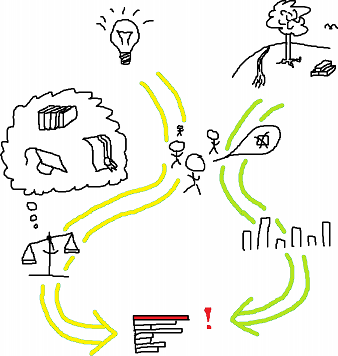
\includegraphics[width=0.75\textwidth]{gfx/speciosgraph2_small.png}
\end{center}
\end{figure}

Mit Hilfe des Wahlsystemes entscheidet jedes Mitglied über grundlegende Dinge und Daten bzw. definiert sie, siehe \vref{fig:choices}. Daraus baut das System mit Hilfe von ebenfalls gewählten einfachen Formeln oder komplexen Skripten diverse Zusammenhänge zwischen den Daten auf, welche mit Hilfe einer künstlichen Intelligenz (siehe \vref{sec:ki}) möglichst effektiv zu Regeln und Handlungsempfehlungen synthetisiert werden.

Es können verschiedene Daten zum selben Sachverhalt eingetragen werden, wobei jedes Datum an mindestens ein Mitglied gebunden ist. Dadurch wird eine dynamische Abstimmung zu jedem Sachverhalt ermöglicht.

Zum Schutz vor Fehlinformationen aufgrund von Unwissenheit oder Meinungen aus dem Bauchgefühl heraus, gibt es zwei Lösungen: Zum einen werden vom System abstrahierte Sachverhalte, welche auf spezielleren, grundlegenderen Daten beruhen, höher bewertet als allgemeine Aussagen. Zum anderen werden die Qualifikationen des Wählers berücksichtigt, welche zur Erfassung des jeweiligen Sachverhaltes benötigt werden (Kompetenzwichtung). Diese werden von anderen Mitgliedern (z.B. Lehrern, Professoren udgl.) geliefert und müssen verifiziert werden, bzw. ergeben sich aus Zeugnissen oder sonstigen Leistungsnachweisen.

\subsubsection{Benutzerschnittstelle}

In einer persönlichen Übersicht wird jedes Mitglied einsehen können, welche seiner Eingaben nicht mit den aktuellen Festlegungen übereinstimmen, um sie ggf. zu korrigieren oder die entsprechende Stimme zu entfernen. Umgekehrt werden "`unsichere"' Daten, die zwar auf mehrheitlichen oder fundamentaleren Ansichten basieren, aber (soweit möglich automatisch korrigierte) Konflikte mit anderen Daten aufweisen oder eine nicht zu vernachlässigende Menge an Gegenmeinungen besitzen, hervorgehoben, damit strukturelle Fehler, neue Erkenntnisse oder alternative Betrachtungen Aufmerksamkeit erhalten.

\subsubsection{Durchmischtes}

ich glaub ich mach das so:

1) daten oder datenblöcke (intern dasselbe, aber der verbund muss wiedererkennbar sein, um blockweise wahlen zu ermöglichen) über alles mögliche, aber immer mit orts-, zeitraum- und genauigkeits-angaben können von jedem benutzer über spezielle webinterfaces oder über eine API eingetragen werden. jeder benutzer kann daten über dieselbe sache in derselben orts- und zeit-ebene nur 1x im system haben, darf sich auch nicht überschneiden. wenn ein benutzer die daten einer anderen person wählt, ist das logisch (und vielleicht auch technisch) dasselbe als würde er eben diese daten von sich aus einfügen.

2) auf magische weise werden dann mehrheits- und kompetenzgewichtungen reingeworfen, überschneidungen und konflikte aufgelöst (besonders lustig bei zahlendaten) und am ende stehen dann die besten vorschläge da.

3) in einem schritt, vielleicht demselben, werden dann konflikte zwischen abstraktionsschichten irgendwie aufgelöst, diese überhaupt zu finden ist vielleicht auch nicht gerade einfach. und untere schichten müssen auf alle oberen vereinfacht werden.

4) ein problem ist bei dem ganzen kram, dass bestimmte operationen vorzugsweise unmittelbar vom system bearbeitet werden müssen, z.b. übersetzungen von wörtern müssen sofort übernommen werden, das einfügen neuer daten sollte sofort sichtbar sein, usw.

5) und dann kommt die richtige magie, lauter demokratisch ermittelte scripte, die zusammenhänge zwischen den rohdaten herstellen und höhere tatsachen definieren. z.b. die wichtigkeit der spezies mücke bezogen auf dessen intelligenz und der anzahl lebender exemplare in deutschland oder so. diese scripte generieren also neue daten, die die "richtigkeit" der baiserenden daten mit einbeziehen muss, damit falls sie neue daten definieren für die es bereits manuelle meinungen gibt, wieder neu entschieden werden kann was denn nun korrekt ist - klingt kompliziert.

6) und zum schluss muss specios aktions-skripte und dessen auswirkungen über die zeit simulieren, um zu ermitteln wie am ende die basisziele maximal erfüllt werden. für einen gedanken muss ggf. alles ab punkt 3 wiederholt werden. ungenaue aber schneller ableitbare folgen mit entsprechend schlechteren wahrscheinlichkeiten erhöhen dabei die arbeitsgeschwindigkeit, also muss der kompromisse zwischen zeit, genauigkeit und wichtigkeit fällen.

\subsection{Sicherheit}\label{sec:maintenance/security}

Vor Manipulationen kann man sich mit Hilfe verteilter Gegenrechnungen, zertifizierter Systemschnappschüsse und spezieller Notpläne schützen. \myindexednote{Notpläne}Mit Notplänen sind (gedruckte) zertifizierte Repräsentationen der wesentlichen abstrahierten Regeln gemeint, welche in jedem Haushalt oder ähnlichen, möglicherweise größeren Gruppierungen gehalten und durch einen sicheren, möglichst persönlichen Mehrheitsentscheid aktiviert werden können. Schnappschüsse und Notpläne besitzen eine zeitlich begrenzte Gültigkeit, um dem Missbrauch von nachträglich entdeckten Gesetzeslücken vorzubeugen.

\section{Künstliche Intelligenz}\label{sec:ki}

Die künstliche Intelligenz (KI) muss die Folgen möglicher Tätigkeiten simulieren und daraus notwendige Handlungen berechnen. Da dies ziemlich rechenaufwendig ist, besteht das Hauptproblem darin, einen Kompromiss zwischen Prioritäten, Zeit und Abstraktionsebene zu finden und Berechnungen je nach Notwendigkeit nach und nach verfeinern und optimieren zu können. Die vorrausschauende Planung der notwendigen Berechnungen ist dabei von zentraler Bedeutung.

Die Arbeitsweise kann in folgende Prozesse eingeteilt werden:
\medskip
\begin{compactitem}
\item Wahlprozess (siehe \vref{sec:maintenance/voting})
\item Konfliktkorrekturprozess
\item Zusammenführungsprozess
\item Auswertungsprozess
\item Abstrahierungsprozess
\item u.\,a.
\item Simulationsprozess
\end{compactitem}
\medskip

Die verschiedenen Prozesse werden im Folgenden näher beschrieben.

\subsection{Simulationsprozess}\label{sec:ki/simulation}

Die KI führt Effizienz"=Abschätzungen durch, wobei für mögliche Tätigkeiten und Betrachtungen jeweils die Wahrscheinlichkeit berechnet wird, wie zielführend eine nähere Untersuchung sein wird. Im Endeffekt wird fortwährend versucht die erwartete Wahrscheinlichkeit, Grundgesetze einzuhalten, und variable Systemparameter (wie der Wohlstand von Systemmitgliedern und anderen Lebewesen, siehe dazu \vref{sec:basis/aim}) auf lange Sicht zu maximieren.

Dazu werden mögliche Aktionskombinationen nicht willkürlich durchprobiert, sondern sie werden anhand der Zieldefinitionen und diverser Wahrscheinlichkeitsfaktoren errechnet und dynamisch verfeinert, so dass das System jederzeit mit der maximal denkbaren Fortschrittsgeschwindigkeit läuft. Um wegen chaotischem Verhalten von Aktionen oder Fehlern nicht fehlgeleitet zu werden, werden suboptimale Lösungswege sowie zufällig gewählte parallel analysiert, je nach Priorität der Kernanalyseaufgaben.

\subsubsection{Daten}

Viele Daten besitzen zusätzlich Orts"~, Zeit"~/""Gültigkeits"~ und Genauigkeits"=Angaben.

\subsubsection{Durchmischtes}

ich glaube die implementierung von specios würde einer ki wie wir sie bisher halbwegs geplant haben ziemlich nahe kommen müssen:
z.b. muss es informationen verallgemeinern können (aus effizienzgründen), abschätzen welchen fehler informationen haben und ggf. spezialisieren/neu berechnen. dafür muss es aber hoffentlich nicht unbedingt informationen in zusammenhang setzen oder neue informationen ableiten, das ist ja mehr oder weniger der demokratische akt: meinungen sammeln, zusammenhänge aufbauen, gesetze formulieren. das system zeigt quasi nur auf abstrakter weise auf was sache ist und was getan werden muss.
und es muss aktivitäten simulieren, was auswirkungen auf sämtliche daten hat und erkenntnisse zulässt.
das hauptproblem neben der spezifikation ist vermutlich der denkvorgang mit dem beschränkten arbeitsspeicher.

\section{Datenbanksystem}\label{sec:database}

Es ist ein dokumentbasiertes Datenbanksystem erforderlich, bei dem jeder Datenpunkt durch eine Datei repräsentiert wird. Aufgrund der Menge an Daten ist ein kompliziertes Verwaltungssystem erforderlich, welches einfach überschaubar und handhabbar ist. Sämtliche Hilfssysteme wie ein Indizierungssystem müssen optional sein. D.\,h. das Datenbanksystem muss sich bei Problemen vollständig selbst rekonstruieren können, sofern die jeweilige Datendateien oder Sicherungen von Ihnen zugänglich sind.

\chapter{Sonstiges}\label{chap:misc}

\section{Geschichte}\label{sec:history}

\begin{itemize}[zwischen 2003 und 2006:]
\item[zwischen 2003 und 2006:] Initiale Ideensammlung zum perfekten politischen System.
\item[15.03.2007:] Die Idee zu DADD (Demokratische AutoDiktatur Deutschland)\footnote{Urheber will nicht genannt werden.} ist entstanden.
\item[25.03.2007:] Die Idee zu Specios ist entstanden.
\item[19.07.2010:] Erste Konzept"=Formulierung.
\item[ab August 2010:] Webseitenentwicklung und nähere Analysen zur technischen Umsetzung.
\end{itemize}
\section{Meilensteine}\label{sec:milestones}

\begin{enumerate}[1.]
\item Ausarbeitung des Konzeptes.
\item Strukturiertes System zur Erstellung und Bewertung von Inhalten.
\item Automatische Ableitung von höheren Zielen, Regeln u.\,ä. anhand der elementaren Entscheidungen.
\item Zuverlässige Repräsentation des Meinungsbildes der Bevölkerung.
\item Adaption der Politik an diese Regeln.
\item Stabiles und sicheres Konzept zur Wahrung des Supera Specios.
\end{enumerate}

\section{Schlusswort}\label{sec:conclusion}

Im Endeffekt erhält man mit Specios ein mögliches System nach dem man sich richten kann, oder eben nicht. Man wird jedoch feststellen, dass sein Wohlbefinden durch dieses System am besten sichergestellt werden kann und es deshalb jedem anderen vorziehen -- auch wenn man die o.\,g. Grundlagen noch nicht ganz unterschreiben möchte.

\appendix


\listoffigures
%\listoftables
\printindex

%\begin{thebibliography}{BGW/VKU, 2007}
   %\bibitem[BGW, 2006]{bgwp20068}\textsc{Bundesverband der deutschen Gas- und Wasserwirtschaft} (2006): \textit{Leitfaden SLP. Praxisinformation P 2006/8 Gastransport/Betriebswirtschaft: Anwendung von Standardlastprofilen zur Belieferung nicht"=leistungsgemessener Kunden.}
   %\bibitem[BGW/VKU, 2007]{bgwvkup200713}\textsc{Bundesverband der deutschen Gas- und Wasserwirtschaft; Verband kommunaler Unternehmen e. V.} (2007): \textit{Praxisinformation P2007/13 Gastransport/Betriebswirtschaft: Abwicklung von Standardlastprofilen.}
   % \bibitem[BMBF, 2003]{bmbf}"'IT-Ausstattung der allgemein bildenden und berufsbildenden Schulen in Deutschland"', http://www.schulen-ans-netz.de/neuemedien/fakten/dokus/it-ausstattung-2003.pdf, 10.03.2005
%\end{thebibliography}
\bibliography{main}

\end{document} 